
\section{Model validation and comparison}

As previous chapter selects the top candidate(s) from three family of models, this chapter describes the full validation of the models and report the most notable results from the process.

\begin{figure}[h]
    \centering
    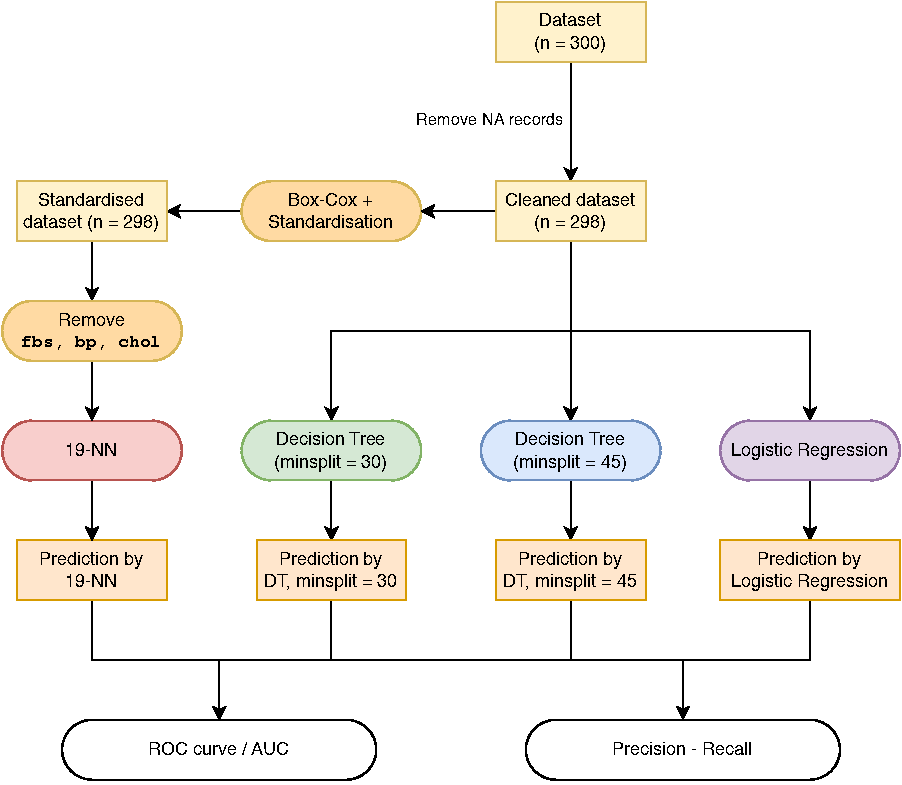
\includegraphics[width=\linewidth]{40.Validation-Diagram.pdf}
    
    \caption{\centering Process of models validation}
\end{figure}

The data pipeline starts with a full dataset of \( n = 300 \) records, two of which with unrecorded fields are then removed. A derivation of the dataset is generated by applying Box-Cox transformation and standardisation to all features, regarding categorical values as if they were numerical. The derived dataset is then fed to the \( 19 \)-NN model for training, whilst other models (logistic, decision trees) are given the cleaned, untransformed dataset. Each model produces a corresponding prediction result, which are then evaluated on the basis of (a) ROC-curve / AUC-score and (b) Precision — Recall curve.




\subsection{ROC - AUC (Receiver Operating Characteristic curve and Area Under the Curve)}

\begin{figure}[H]
    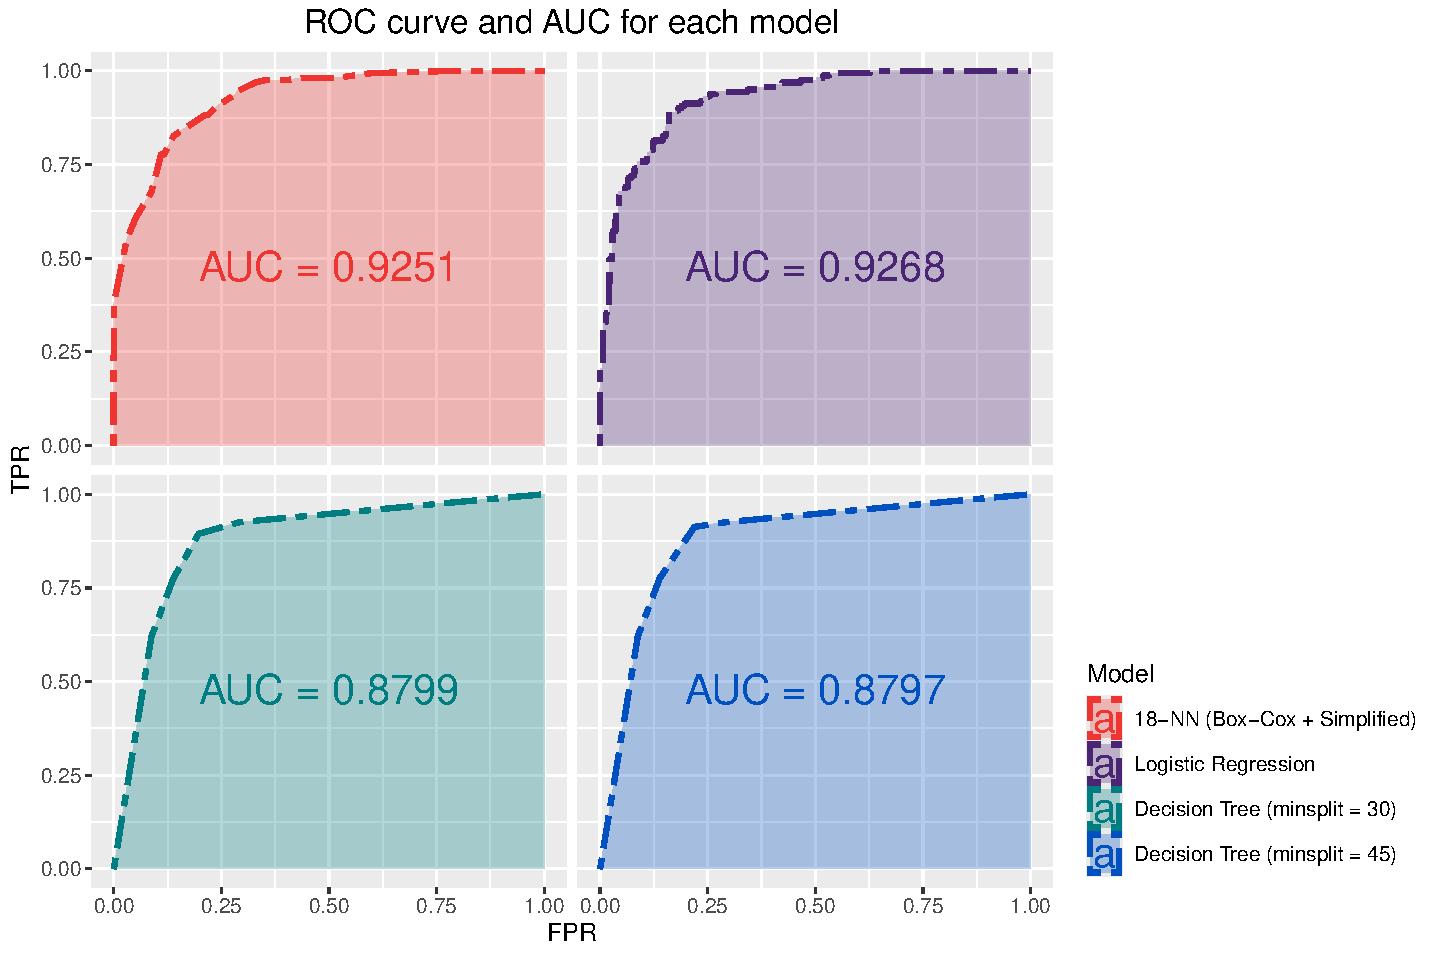
\includegraphics[width=\linewidth]{40.ROCs.pdf}
    \caption{\centering ROC curves and AUC for each model}
\end{figure}

Surprisingly, \( 19 \)-NN and logistic model produce similar ROC curves, despite having different modelling methodologies. It is less so for decision trees, as their alike curves can be explained by the analogous inner mechanisms of their structure.

In terms of AUC score, \( 19 \)-NN and logistic model give impressive scores of \( 0.9245 \) and \( 0.9268 \) respectively, whilst decision trees only yield less impressive scores from \( 0.8797 \) to \( 0.8799 \). The former models excel by considering exhaustive combinations of features, whilst the latter models suffer from overgeneralisation by only considering the most important features and skipping the details.





\subsection{Precision - Recall (TPR)}
\begin{figure}[H]
    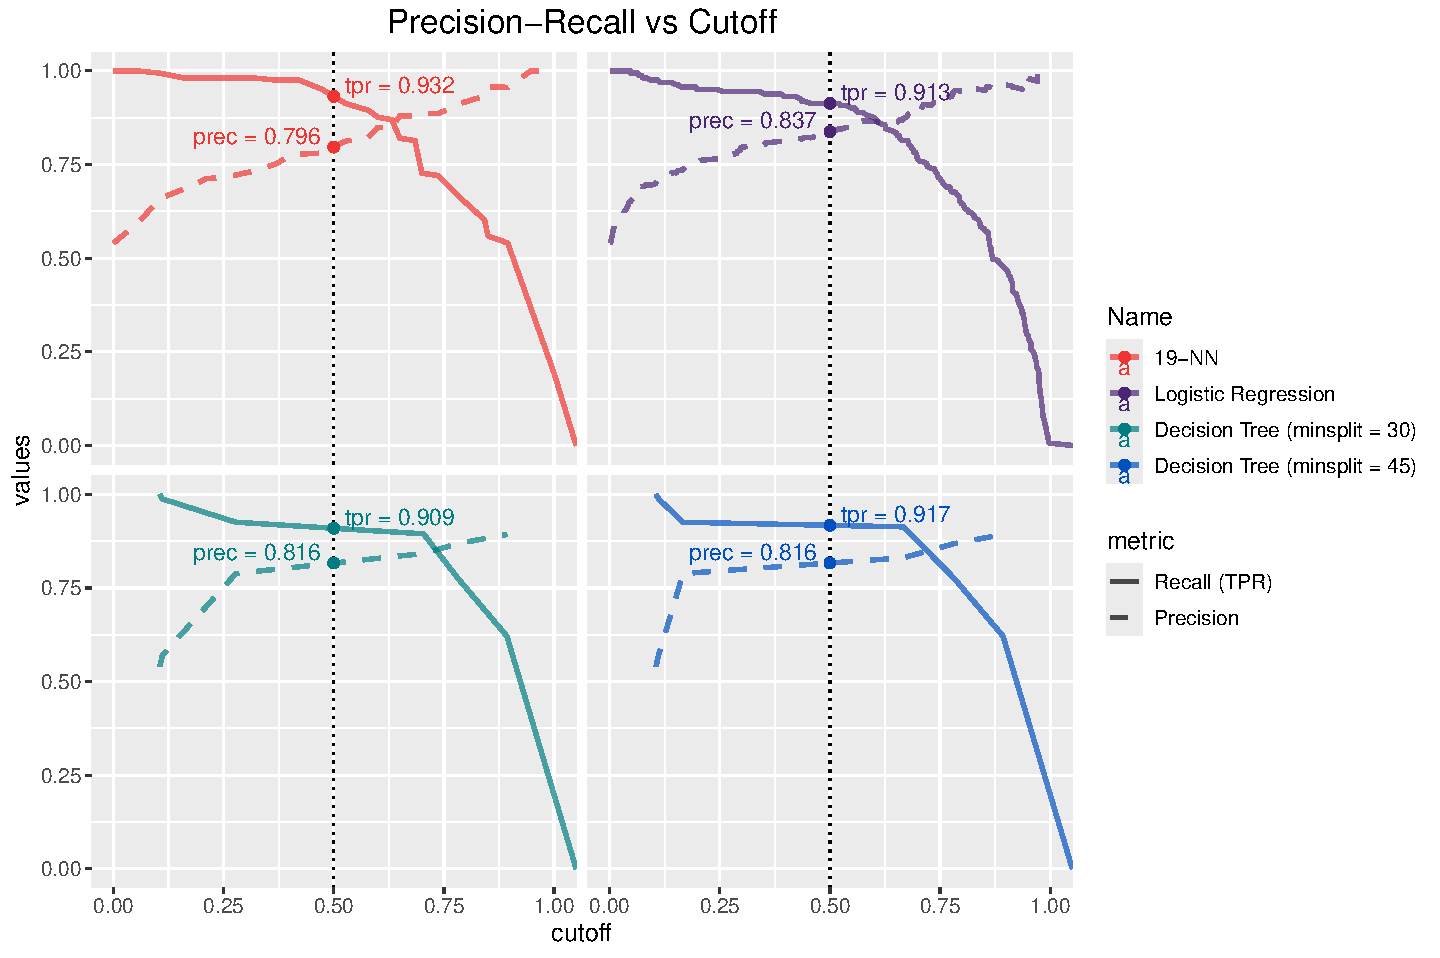
\includegraphics[width=\linewidth]{40.TPRs.pdf}
    \caption{\centering Percision/Recall -- Cutoff curves for each model}
\end{figure}

As the cutoff threshold increases, precision increases gradually whilst recall (TPR) decreases substantially, especially after the \( 0.5 \) threshold. Comparing models at the standard threshold of \( \delta = 0.5 \), it is observed that no models outperform the others in terms of precision and recall. \( 19 \)-NN tops at a \( 0.932 \) recall but fails at a low \( 0.796 \) precision, whilst logistic model observes a humble \( 0.913 \) recall but an impressive \( 0.837 \) precision. Decision trees are somewhat in between, with the \(45\)-minsplit model having a moderate \( 0.917 \) recall and \( 0.816 \) precision. 

\begin{figure}[h]
    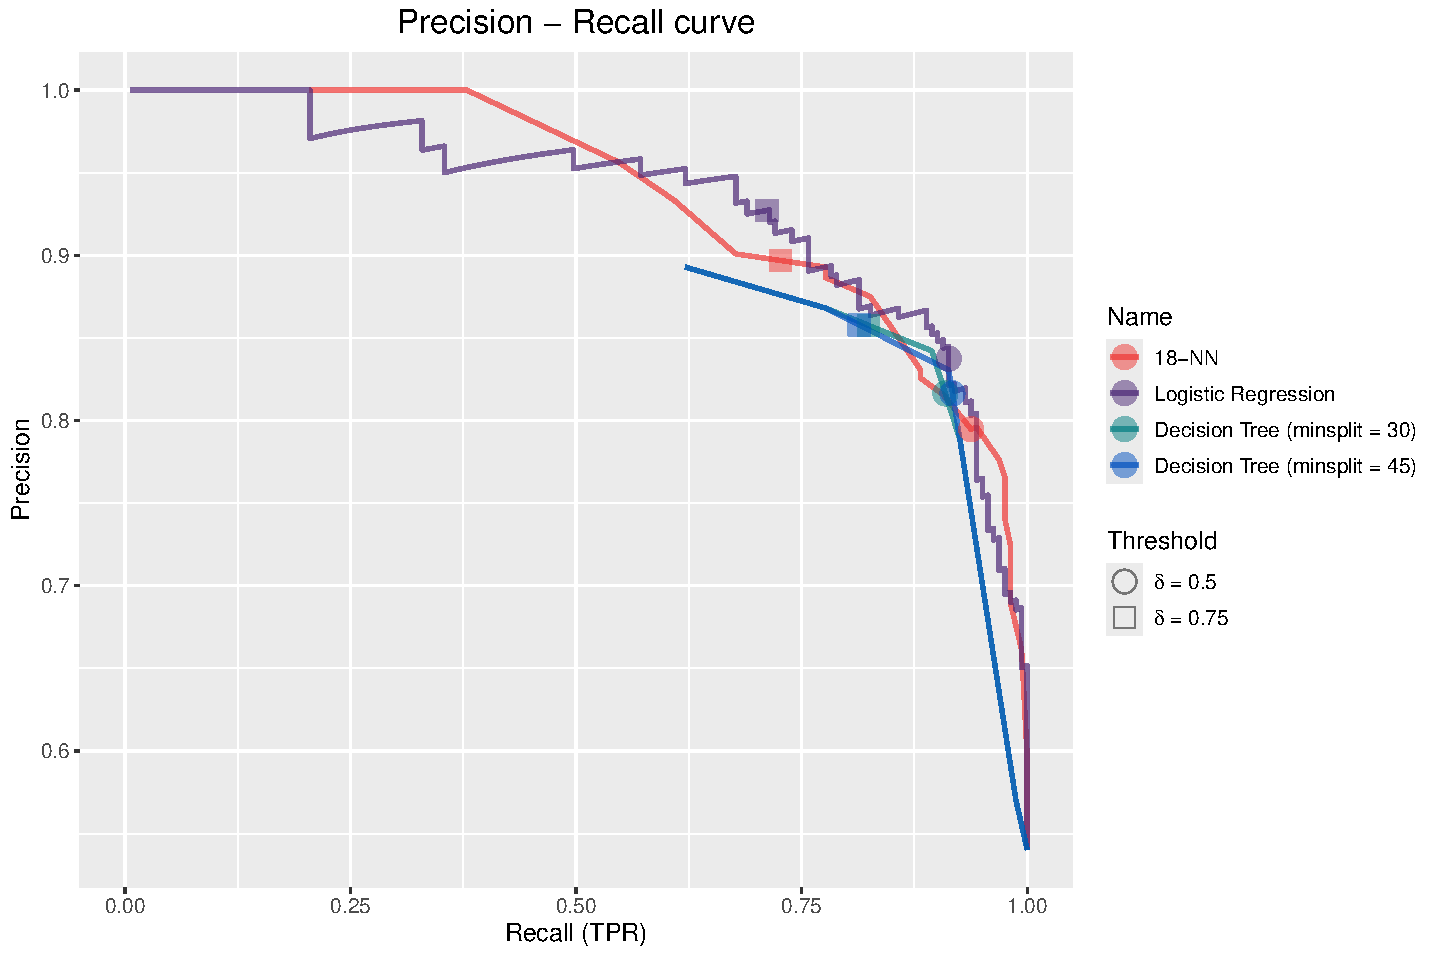
\includegraphics[width=\linewidth]{40.Precision-Recall.pdf}
    \caption{\centering Percision -- Recall curve}
\end{figure}

As the threshold is moved to \( \delta = 0.75 \), decision trees perform better in recall whilst logistic model and \( 19 \)-NN improve in precision. Concaveness around the \( \delta = 0.75 \) threshold is observed on the precision-recall curve of the \( 19 \)-NN model, whilst logistic model generally still performs well around this region.

